\documentclass[10pt,twocolumn,letterpaper]{article}

\usepackage{cvpr}
\usepackage{times}
\usepackage{epsfig}
\usepackage{graphicx}
\usepackage{amsmath}
\usepackage{amssymb}
\usepackage{pdfpages}
\usepackage{gensymb}

%%%%%%%%%
% Example of figure inclusion
%\begin{figure}[t]
%\begin{center}
%\fbox{\rule{0pt}{2in} \rule{0.9\linewidth}{0pt}}
%   %\includegraphics[width=0.8\linewidth]{egfigure.eps}
%\end{center}
%   \caption{Example of caption.  It is set in Roman so that mathematics
%   (always set in Roman: $B \sin A = A \sin B$) may be included without an
%   ugly clash.}
%\label{fig:long}
%\label{fig:onecol}
%\end{figure}

%%%%%%%%%
% Example table
%\noindent
%Compare the following:\\
%\begin{tabular}{ll}
% \verb'$conf_a$' &  $conf_a$ \\
% \verb'$\mathit{conf}_a$' & $\mathit{conf}_a$
%\end{tabular}\\
%
%
%
%\begin{table}
%\begin{center}
%\begin{tabular}{|l|c|}
%\hline
%Method & Frobnability \\
%\hline\hline
%Theirs & Frumpy \\
%Yours & Frobbly \\
%Ours & Makes one's heart Frob\\
%\hline
%\end{tabular}
%\end{center}
%\caption{Results.   Ours is better.}
%\end{table}

%%%%%%%%%
% another example figure
%\begin{figure*}
%\begin{center}
%\fbox{\rule{0pt}{2in} \rule{.9\linewidth}{0pt}}
%\end{center}
%   \caption{Example of a short caption, which should be centered.}
%\label{fig:short}
%\end{figure*}
%
%
%%%%%%%%%
% example citation
%   Frobnication has been trendy lately.
%   It was introduced by Alpher~\cite{Alpher02}, and subsequently developed by
%   Alpher and Fotheringham-Smythe~\cite{Alpher03}, and Alpher \etal~\cite{Alpher04}.''

    %Figure and table captions should be 9-point Roman type as in
    %Figures~\ref{fig:onecol} and~\ref{fig:short}.  Short captions should be centred.
% Include other packages here, before hyperref.

% If you comment hyperref and then uncomment it, you should delete
% egpaper.aux before re-running latex.  (Or just hit 'q' on the first latex
% run, let it finish, and you should be clear).
%
% When placing figures in \LaTeX, it's almost always best to use
% \verb+\includegraphics+, and to specify the  figure width as a multiple of
% the line width as in the example below
% {\small\begin{verbatim}
%    \usepackage[dvips]{graphicx} ...
%       \includegraphics[width=0.8\linewidth]
%           {myfile.eps}
%   \end{verbatim}
% }
%
\usepackage[breaklinks=true,bookmarks=false]{hyperref}

\cvprfinalcopy % *** Uncomment this line for the final submission

\def\cvprPaperID{****} % *** Enter the CVPR Paper ID here
\def\httilde{\mbox{\tt\raisebox{-.5ex}{\symbol{126}}}}

% Pages are numbered in submission mode, and unnumbered in camera-ready
%\ifcvprfinal\pagestyle{empty}\fi
\setcounter{page}{1}
\begin{document}

%%%%%%%%% TITLE
\title{Predicting the Eye Fixations with Prior Knowledge: A Bayesian Learning Architecture}

\author{Lauren Arnett and Chengzhi Mao\\
Columbia University in the City of New York\\
    {\tt\small \{lba2138,cm3797\}@columia.edu}
}

\maketitle

%%%%%%%%% ABSTRACT
\begin{abstract} 
    
    Applications of tracking eye fixation location span from neuroscience and
    the study of human vision to advertising and human computer interaction. By
    creating a model to generate a prediction of where the eye may be most
    attracted to, industries can circumvent the expense of running studies on
    eye-tracking with actual human subjects. We look to improve upon existing
    models of saliency by using Bayesian methods with deep learning techniques.

\end{abstract}

%%%%%%%%% BODY TEXT
\section{Introduction} It is estimated that 80\% of all external sensory input
processed by the human brain is processed by the visual pathway~\cite{Jerath}.
As such, optimizing image layout for processing by the human brain allows for
better information retrieval and retention across the image. Studying how
humans’ eyes move across images is thus relevant for fields from neuroscience
to advertising and  art. Being able to predict where humans are most likely to
look provides a guideline as to whether the image has an effective layout, what
humans are attracted to in viewing art, or how an image should be cropped to
feature the subject. Using an existing dataset of eye movements, we build
a predictive model to generate the most likely fixation locations on a new
image.
%-------------------------------------------------------------------------
\section{Related Work} 

Traditionally, studies on eye movements have been carried out such that
viewers look at images on a monitor while an eye tracker records the
eye-fixations that stay within a threshold angle of movement. This procedure is
very costly, and necessitated formulating a method to predict where users will
look. Thus, models of saliency---the likelihood of a location to attract the
visual attention of a human---developed that are modeled mathematically using
biologically plausible linear filters. For example, linear combinations of
filters for low-level features such as color, intensity, and orientation
filters can be used to compute a total saliency map for an image,
providing a bottom-up understanding of the image~\cite{Itti}.

These models do not account for particular tasks that the viewer may have in
looking at the image, and often do not align with the ground truth fixation
locations. Judd \etal~\cite{Judd} propose using deep learning for this task
rather than deriving mathematical models and show that training from a large
database of eye-tracking data outperforms existing models. K\"ummerer
\etal~\cite{Kummerer} also employ deep learning for predicting fixation
locations, using the AlexNet architecture in \textit{DeepGaze I} and \textit{DeepGaze II}, built upon the VGG-19 network.

Developing a dataset for use by saliency models is also a field of exploration.
Judd \etal~\cite{Judd} creates a dataset of 1003 images with the fixation
locations from 15 viewers each and makes it publicly available. Jiang
\etal~\cite{Jiang} relies on an assumption of eye-mouse coordination---they
simulate recording eye-tracking data with instead recording mouse-tracking data
using Amazon Mechanical Turk. This provides a less expensive and
training-intensive method of developing a simulated saliency map. Finally, the
MIT300 dataset \cite{mitbench} looks to provide a performance benchmark for new predictive
models for saliency, with performance statistics for over 80 models at the time
of writing. 


\section{Dataset}
We make use of two datasets: ImageNet for training our prior and an
eye-fixation dataset for our classifier. 
\subsection{Source for Eye-Tracking Data}
We use an open-source dataset developed at Osnabr\"uck University and the
University Medical Center in Hamburg-Eppendorf \cite{Wilming01, Wilming02}. This dataset comprises images
of many categories, including urban and rural settings, fractals, faces, and
websites. For our purposes, we use the images of urban and rural settings,
which have been taken from the LabelMe dataset \cite{labelme}. Each image in
this category is shown to the viewer for eight seconds, and this category has
the x- and y-coordinates of 70,026 fixation locations for seven observers over
600 images. Figure ~\ref{fig:dataset} shows examples of fixation locations
across the image. 
\begin{figure}
    \begin{center}
        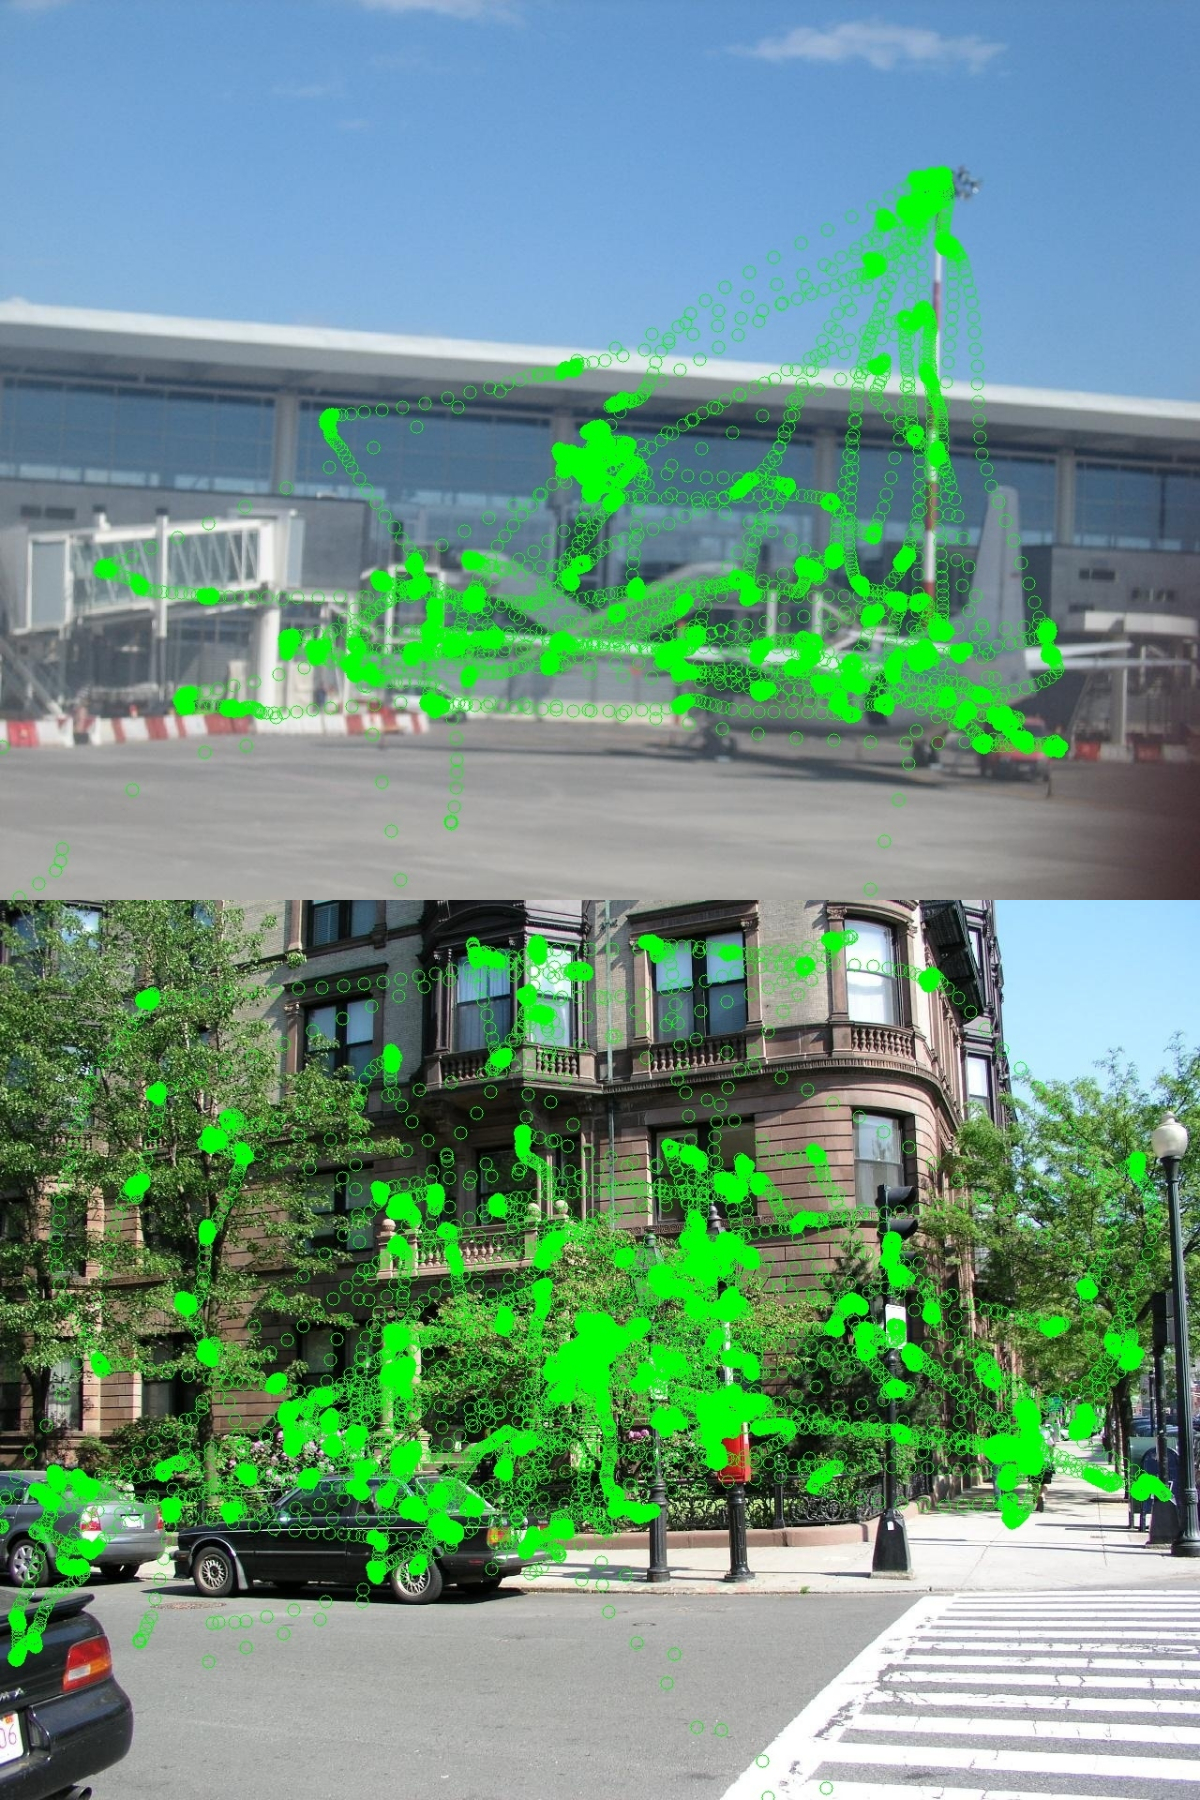
\includegraphics[width=0.5\columnwidth]{figures/movements.jpg}
    \end{center}
    \caption{Eye-tracking locations on sample images from dataset.}
    \label{fig:dataset}
\end{figure}

\subsection{Preprocessing} We preprocess the fixation data by adding weight to
those pixels in the image that have fixations to produce ground truth labels.
We apply a Gaussian blur to also add weight to neighboring pixels to account
for the $0.5\degree$ angle of error due to the eye-tracking machine.
Figure~\ref{fig:preprocess} shows the fixation locations and corresponding
ground truth labels.

\begin{figure}
	\begin{center}
		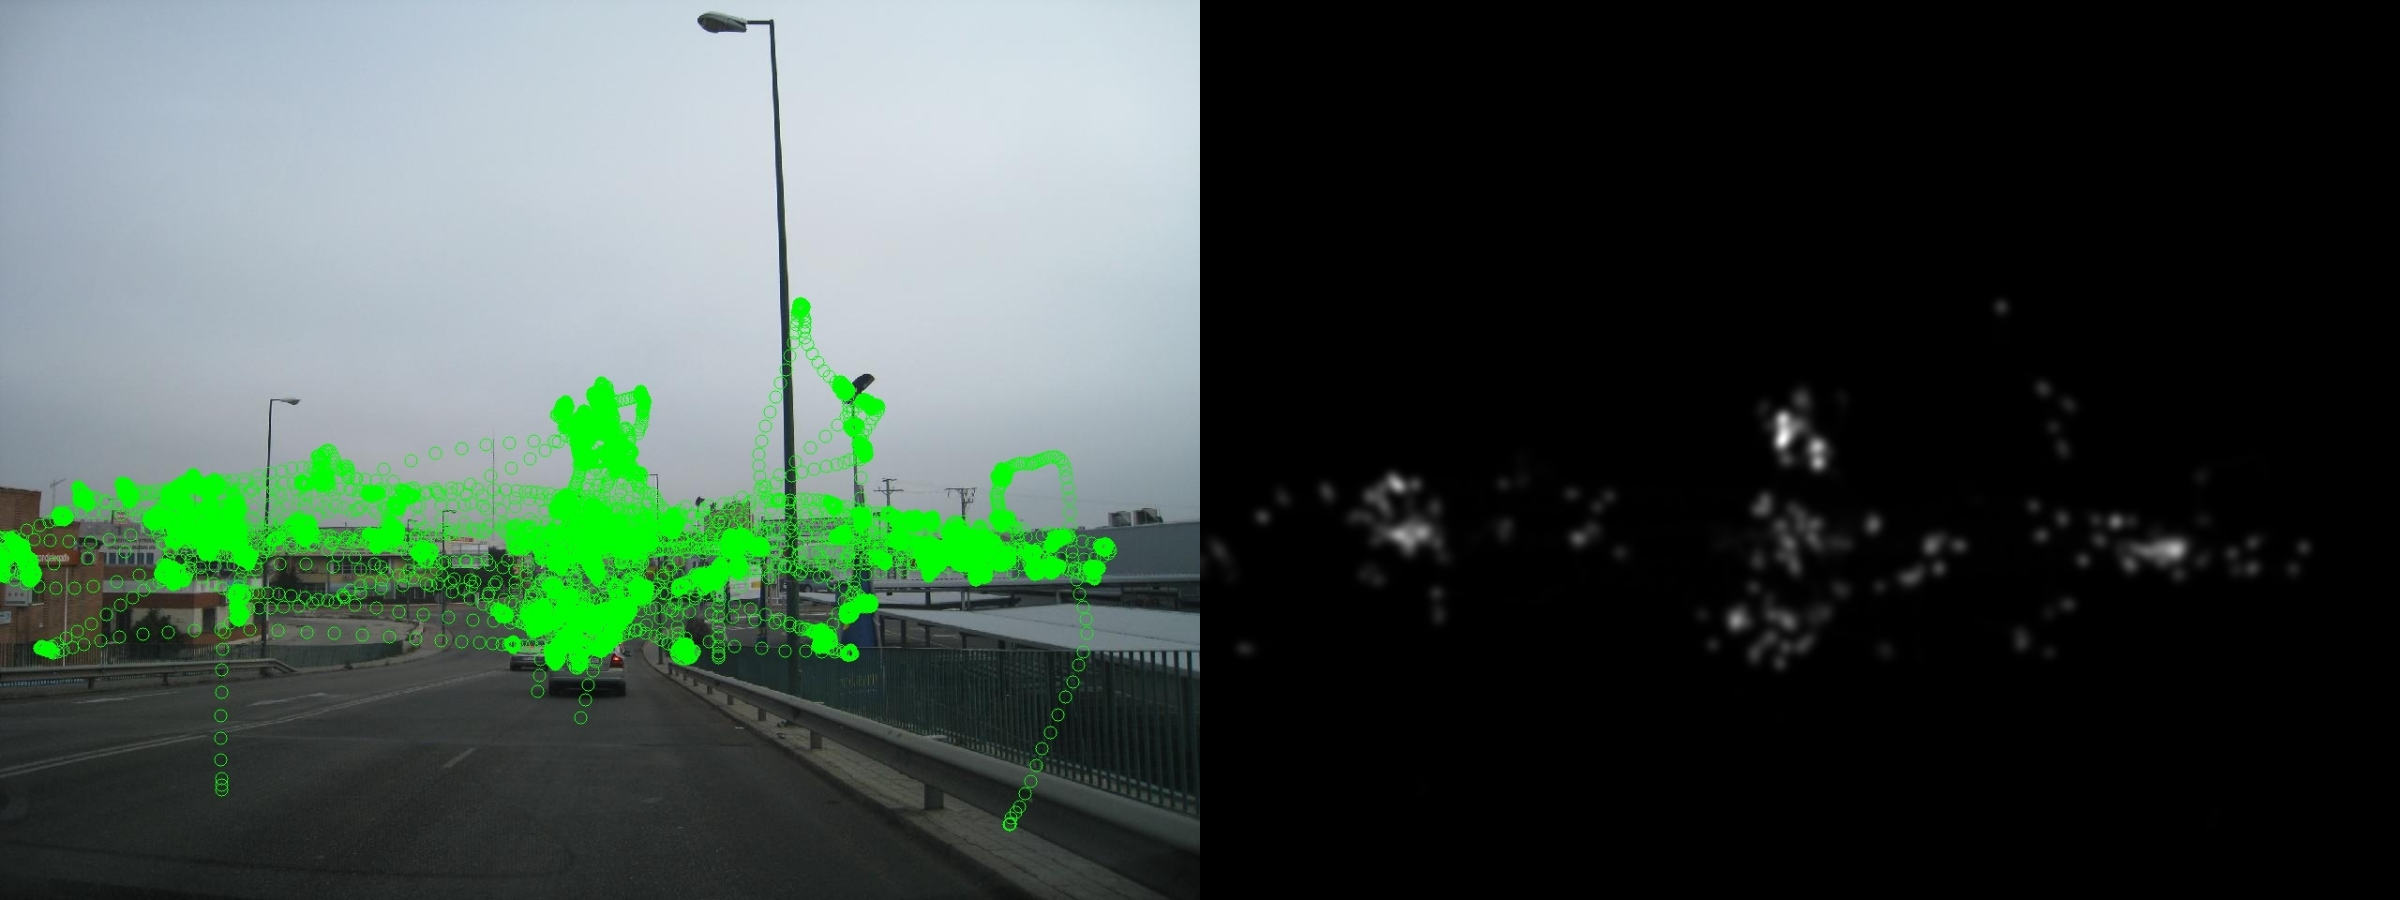
\includegraphics[width=\columnwidth]{figures/preprocess.png}
	\end{center}
	\caption{Preprocessing of the fixation locations.}
	\label{fig:preprocess}
\end{figure}


\section{Learning a Model}
\subsection{Baseline Model Setting}
We conduct a binary classification task for each output pixel in our baseline eye fixation model. We propose a U-Net architecture, using a fixed pretrained VGG model. We take the features of 3, 8, 15, 22 layers in the VGG and feed into our fixation prediction network. We first learn a upsampling of the high level,low resolution features of the VGG, and then concatenate it with the low level, high resolution features.

 \begin{figure}
	\begin{center}
		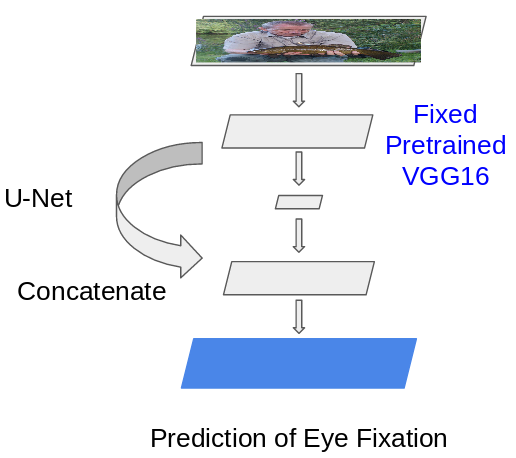
\includegraphics[width=\columnwidth]{figures/architecture_bl.png}
	\end{center}
	\caption{U-Net Architecture for our baseline model}
	\label{fig:unet}
\end{figure}

\subsection{Overcoming the Checkerboard Artifacts of Upsampling}
Building the upsampling using deconvolution operation introduces checkerboard artifacts, as shown in Fig. This is partly due to the overlap of the deconvolution, according to []. We overcome this by first applying a nearest-neighbor interpolation and then normal convolution operation.

\subsection{Learning Prior from the ImageNet}

 Due to the high cost of collecting eye movement data, which requires volunteers to set in front of the computer wearing an eye tracker, the number of samples in the training set is limited. We make an attempt to address this challenges by utilizing some prior knowledge of eye fixation.
 
 \begin{figure}
 	\begin{center}
 		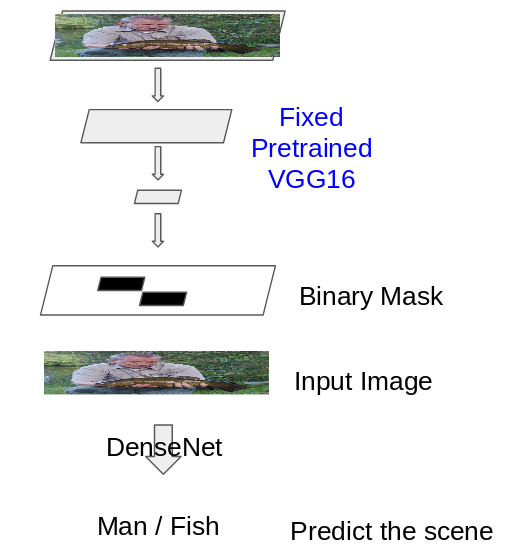
\includegraphics[width=\columnwidth]{figures/Prior.png}
 		
 	\end{center}
 	\caption{Architecture for learning the prior}
 	\label{fig:prior}
 \end{figure}
 
 We interpret eye fixation points as the places which encode the most semantic information for the image. And with this prior, we construct a model which predicts a binary mask with 0 and 1 to select the image, and then use a neural network to predict the semantic information of that after masking image. 
 
 The elements with value 1 in the predicted binary mask mimic the eye fixation point of the human, where the selection of these points should maximize the semantic information in the resulting image after training.
 
 We denote the semantic label of a given image $X$ as $y$, the predicted mask as $M$, and the loss function to minimize $L$
 $$M_i = F_1(X_i, k)$$
 $$L(X, Y) = \sum_{x_i \in X}{logP(y | F_2(M_i * x_i))}$$
 
 where * denotes element wise multiplication, $k$ denote the number of value 1 we need in the binary mask.
 
 After training The $M_i$ can be interpreted as a learned prior knowledge, which is fixed during the bayesian learning scheme.
 
 \subsection{Incorporating Prior Improves Prediction}
 
 The main contribution of our work is a bayesian inference scheme that builds upon a prior knowledge learned externally. We denote the eye fixation ground truth as $t$, 
 
 $$L = logP(M, t|x) = log(P(M|x)) + log(t|M, x)$$
 
 The prior M gives a good estimation of the eye fixation in advance, which enhance the optimization of this loss function.
 
 
 
\subsection{Training}
We train our baseline model using SGD, with learning rate of 1e-5 and weight decay of 1e-6. We train 50 epoch before we stop.

We use ImageNet data for our prior training, where the mask prediction network is based on a pretrained VGG16 network, and the network to predict semantic meaning from the masked out image is a DenseNet, which we believe have more accurate gradient information. We train this Mask prediction network using SGD with learning rate of 1e-5.


\subsection{Performance}

\begin{figure}
\begin{center}
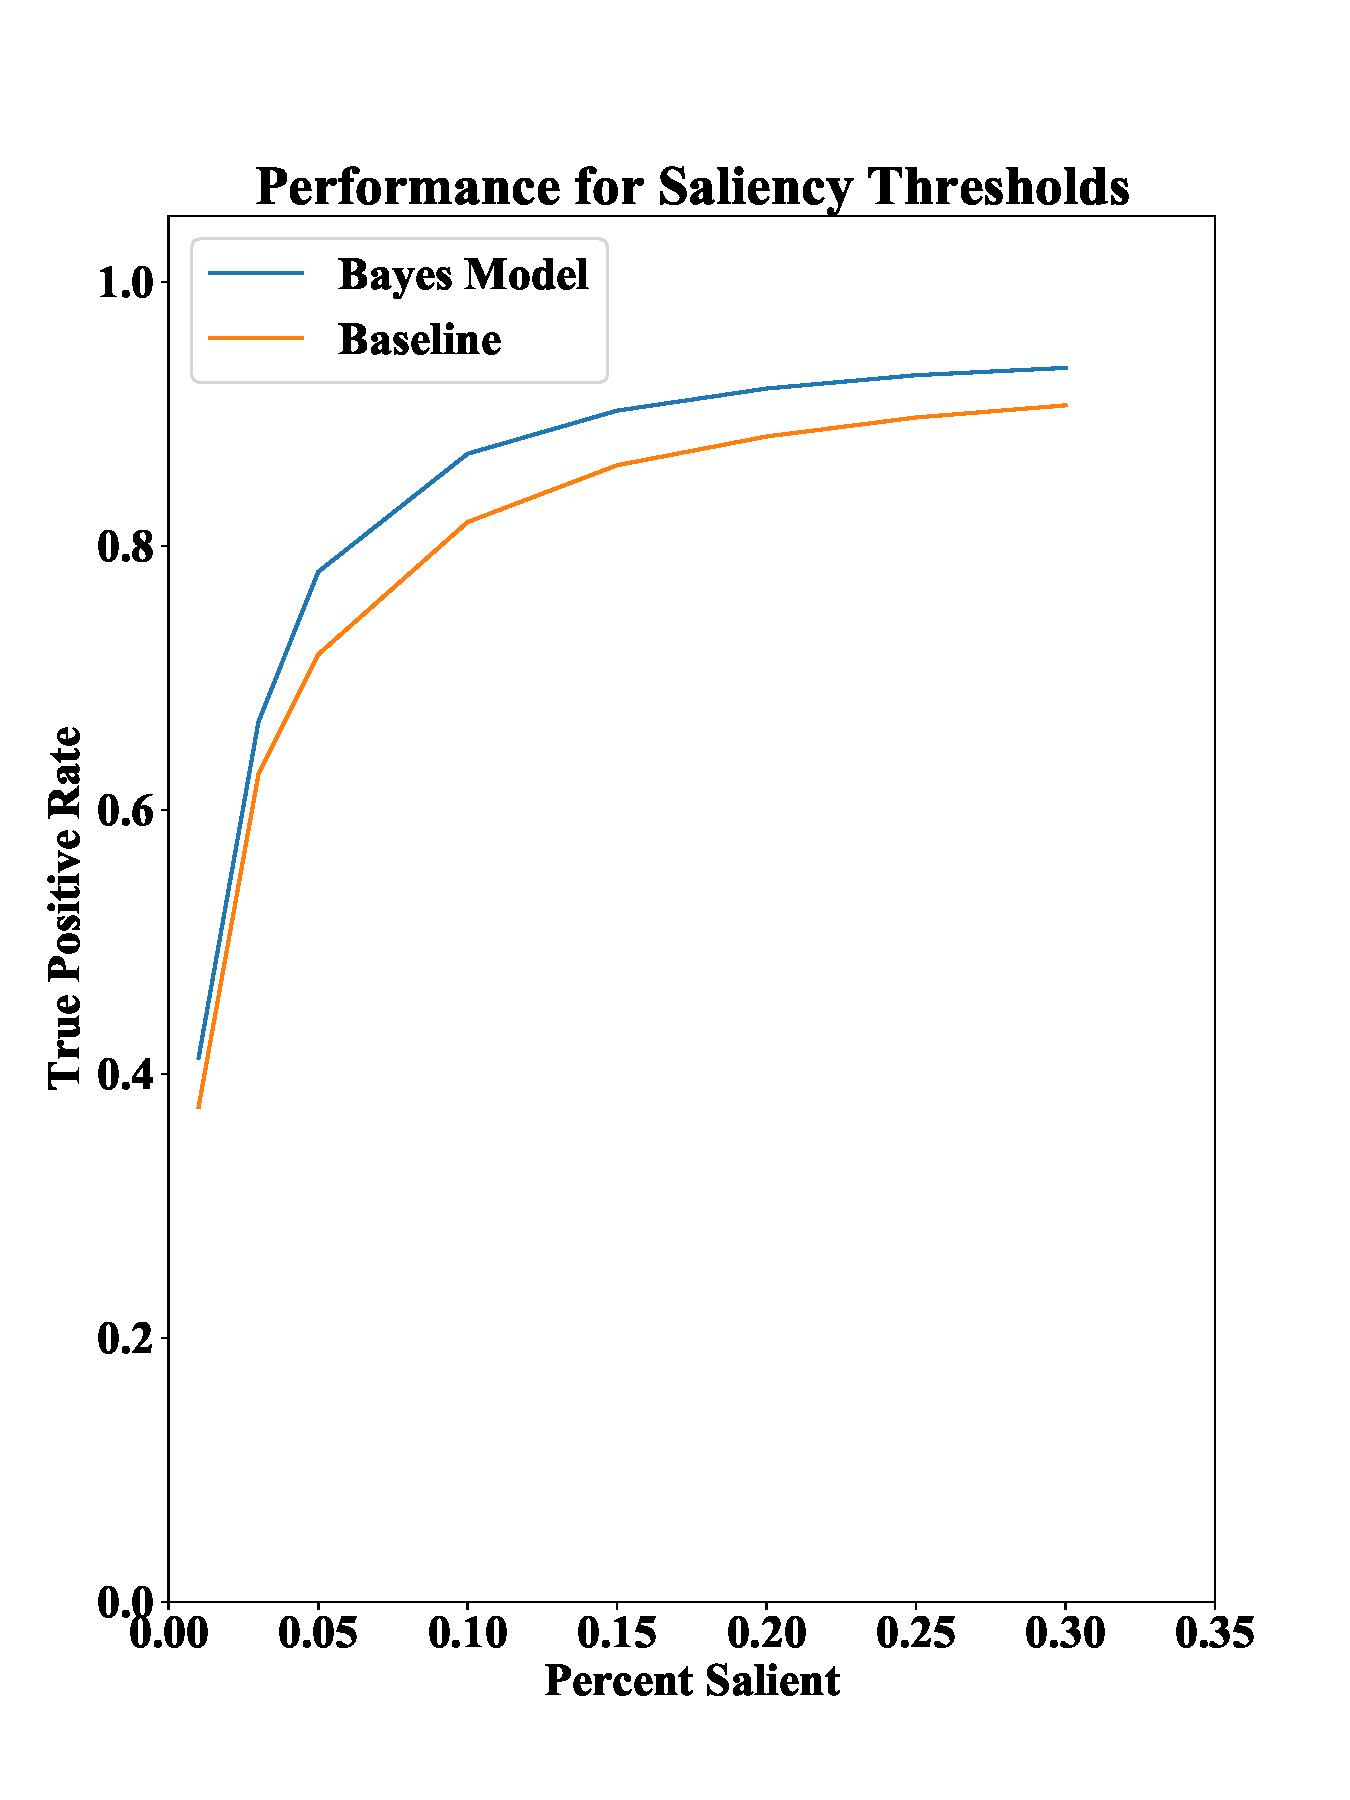
\includegraphics[width=\columnwidth]{figures/tpr.pdf}

\end{center}
   \caption{Example of a short caption, which should be centered.}
\label{fig:short}
\end{figure}


\begin{figure}
	\begin{center}
		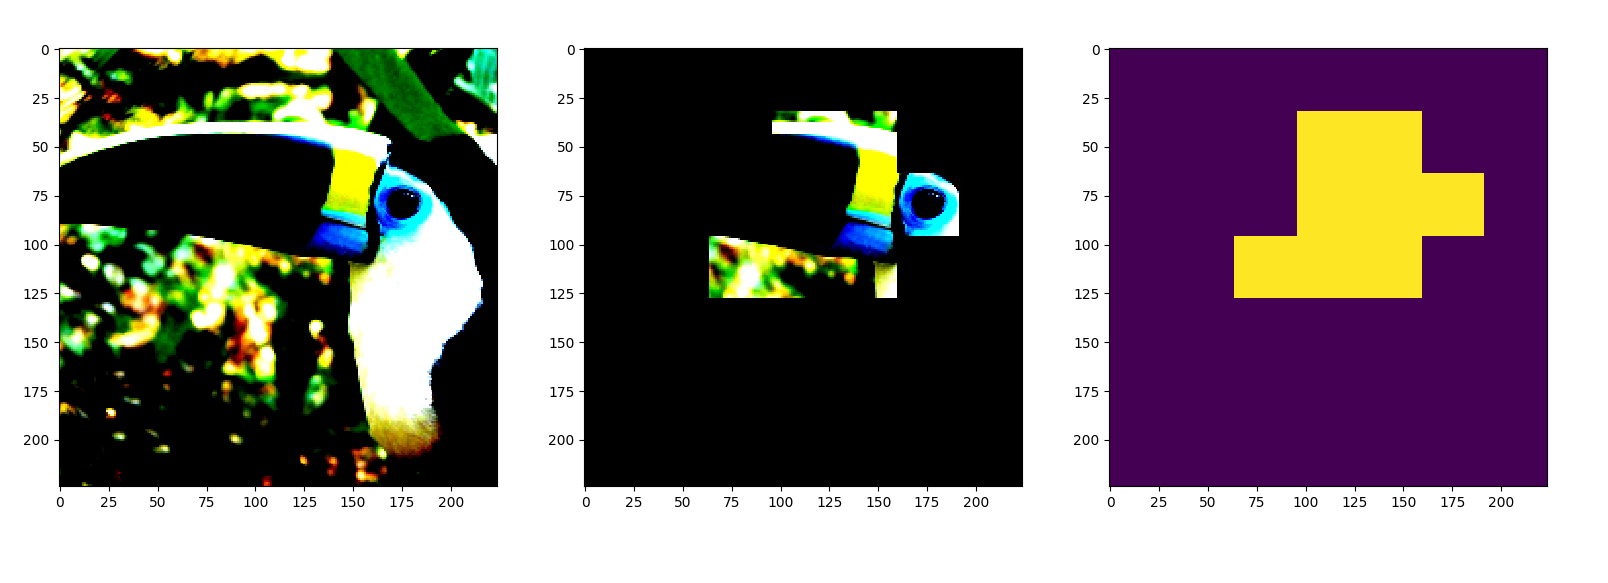
\includegraphics[width=\columnwidth]{figures/bird_mask_predict.png}
		
	\end{center}
	\caption{Example of mask learned on ImageNet}
	\label{fig:short}
\end{figure}

\begin{figure}
	\begin{center}
		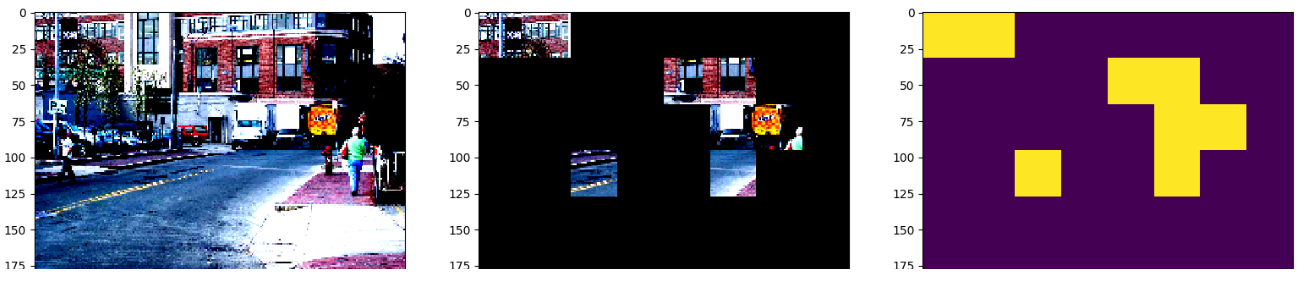
\includegraphics[width=\columnwidth]{figures/road.png}		
	\end{center}
	\caption{Example of extrapolating the prior learned on ImageNet to the eye fixation dataset}
	\label{fig:short}
\end{figure}


\section{Conclusion}

%------------------------------------------------------------------------
{\small
\bibliographystyle{ieee}
\bibliography{egbib}
}

\end{document}
